\subsection{Logic}
Logic indeholder alt logikken i spillet dvs. de metoder som bliver brugt i "Game" klassen til f.eks. at flytte spillerne, købe felter, eller sætte spilleren i fængsel. Derudover holder klassen også styr på hvad der skal til for at vinde spillet og for at finde vinderen af spillet. Klassen bruges også til at skrive bestemt information ud i konsollen. 


\begin{figure}[H]
    \centering
    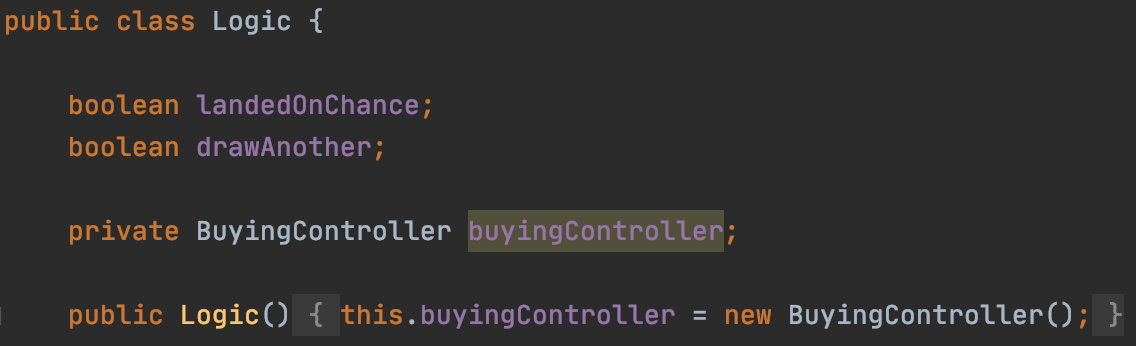
\includegraphics{sources/7_implementering/LogicClass.png}
    \caption{Logic klassen}
    \label{fig:logicClass}
\end{figure}
I klassen har vi defineret to booleans som checker, om man er landet på chance og om man skal trække endnu et kort (drawAnother hører til et bestemt chancekort). Derudover er der en controller til køb og dertil en logic klasse.

\begin{figure}[H]
    \centering
    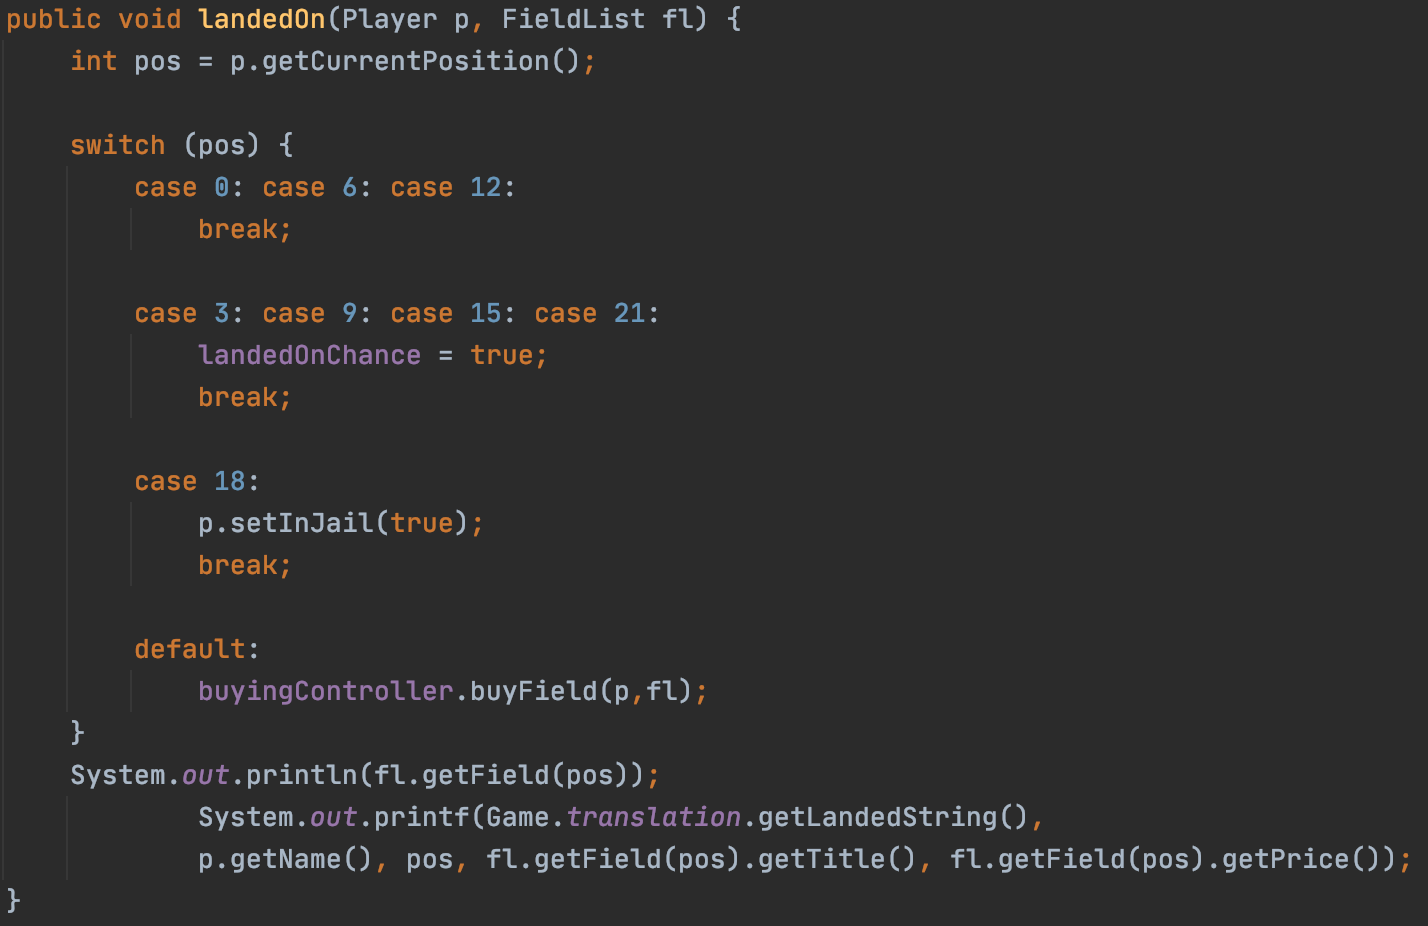
\includegraphics{sources/7_implementering/LogiclandedOn.png}
    \caption{Metoden finder ud af hvilket felt, spilleren lander på}
    \label{fig:logicLandedOn}
\end{figure}
landedOn metoden holder styr på om man er landet på et felt man kan købe, et chancekort eller på fængslet. I så fald vil man blive sat i fængsel, trække et chancekort eller betale for/købe feltet. 



\begin{figure}[H]
    \centering
    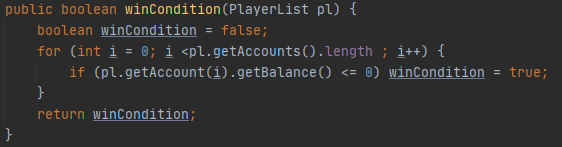
\includegraphics{sources/7_implementering/logic_wincondition.PNG}
    \caption{Når en konto rammer 0}
    \label{fig:logicWinCon}
\end{figure}
winCondition ved, når en spiller har tabt, altså når en konto rammer 0.

\begin{figure}[H]
    \centering
    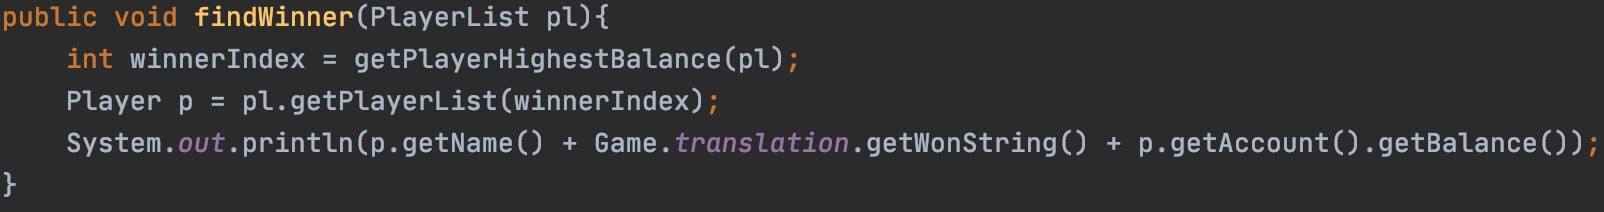
\includegraphics{sources/7_implementering/LogicfindWinner.png}
    \caption{Finder vinderen af spillet}
    \label{fig:logicFindWinner}
\end{figure}
Efter en spiller har tabt, vil metoden her bruge getPlayerHighestBalance metoden og se, hvem der ejer mest. Den vil så erklære vinderen.

\begin{figure}[H]
    \centering
    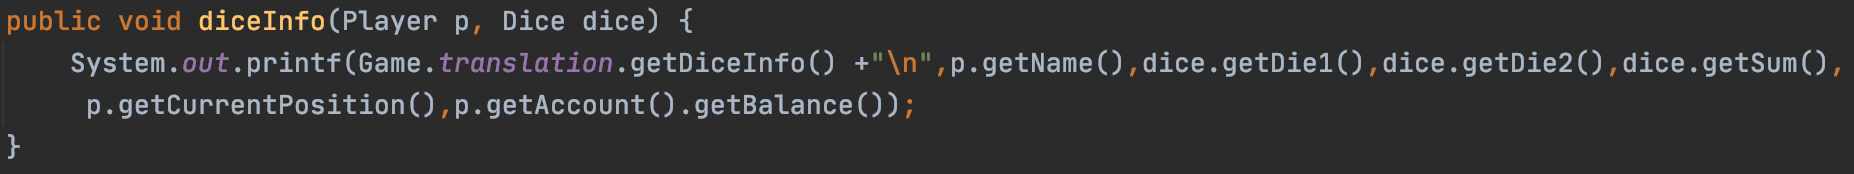
\includegraphics{sources/7_implementering/LogicdiceInfo.png}
    \caption{Metoden viser resultat af terningslag og spillers info efter slag}
    \label{fig:logicDiceInfo}
\end{figure}
diceInfo kalder en række getters . Den får de to terningers øjne og summen af den. Derefter finder den spillerens ny position og kontobeholdning. 

\begin{figure}[H]
    \centering
    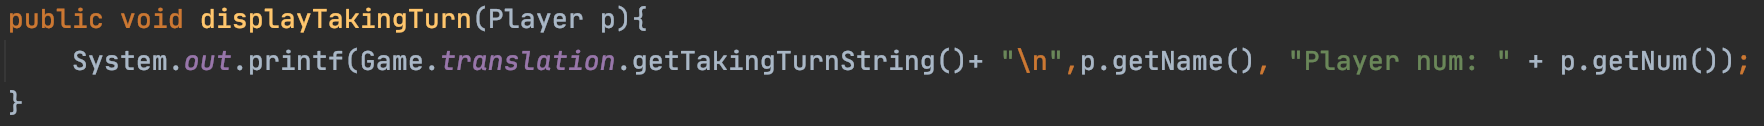
\includegraphics{sources/7_implementering/LogicTakingTurn.png}
    \caption{Kode der beskriver hvordan man vinder}
    \label{fig:logicDisplayTakingTurn}
\end{figure}
displayTakingTurn kender til hvilken spiller, som tager den nuværende tur.

\begin{figure}[H]
    \centering
    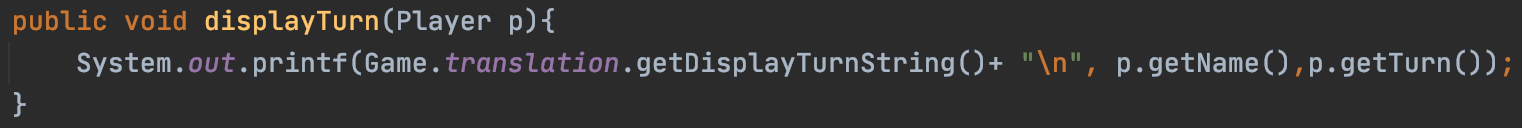
\includegraphics{sources/7_implementering/LogicdisplayTurn.png}
    \caption{Kode der beskriver hvordan man vinder}
    \label{fig:logicDisplayTurn}
\end{figure}
displayTurn fungerer på samme måde og ved hvilken tur, det er.

\begin{figure}[H]
    \centering
    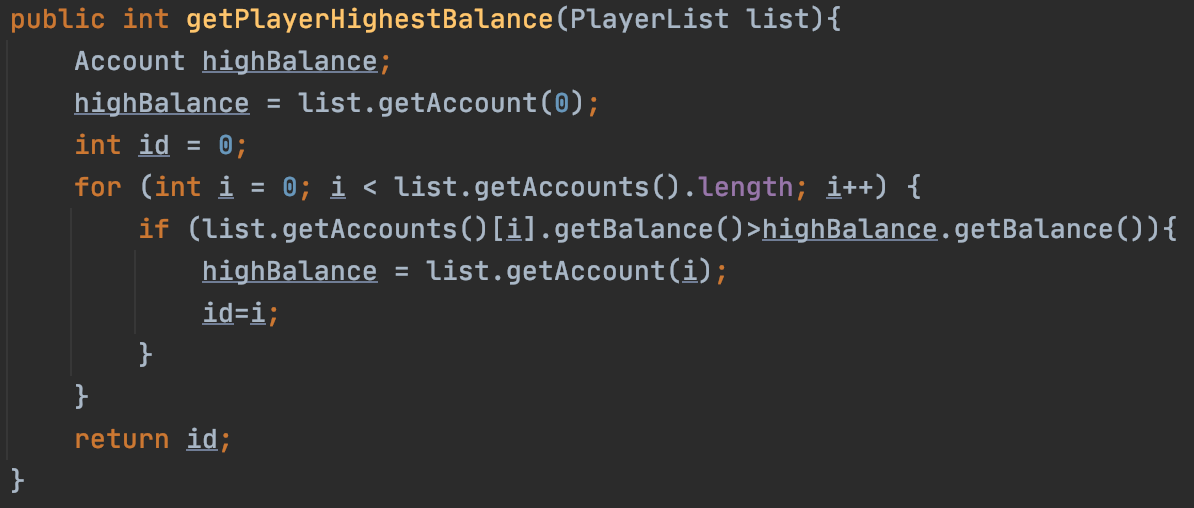
\includegraphics{sources/7_implementering/LogicgetHighestBalance.png}
    \caption{Kode der beskriver hvordan man vinder}
    \label{fig:logicHighestBalance}
\end{figure}
getPlayerHighestBalance bruges til at finde ud af hvilken spiller, der har flest penge på sin konto. Det sker ved et loop, som kigger på alle konti og vælger den med flest penge, som dermed vinder spillet.

